\section{Welcome to Illinois}

\begin{figure}[H]
  \centering
  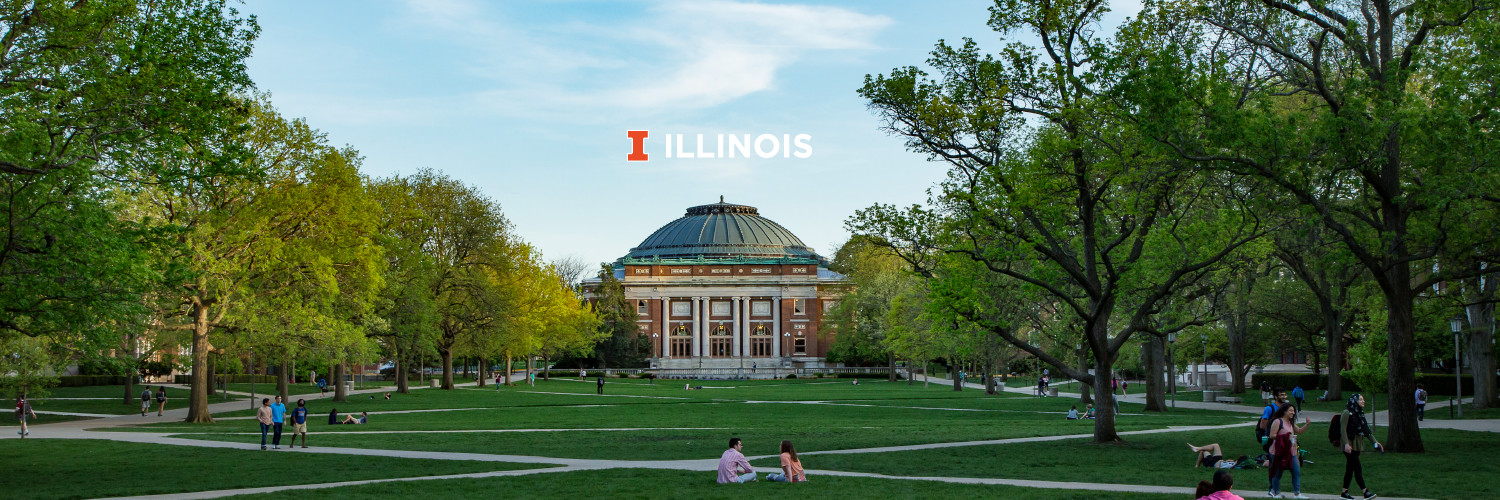
\includegraphics[width=\textwidth]{illinois-main.jpeg}
\end{figure}

\subsection{Champaign-Urbana in a Nutshell}
Champaign-Urbana (CU), colloquially known as Chambana, is home to the state's flagship school, the University of Illinois at Urbana-Champaign (UIUC). Since its founding in the mid 19th century CU has grown into the flourishing cultural hub of the midwest it is today. CU houses many landmarks and districts, and showcases both local and national events annually. It is home to the Historic Virginia Theater that hosts Ebertfest in honor of the late film critic and UIUC alumnus Roger Ebert. The Krannert Center for the Performing Arts is located on U of I campus, which is known for its four first-class venues, including the Foellinger Great Hall - one of the most acoustically perfect performance spaces in the world, attracting world famous artists and ensembles to perform there every year. Other notable events that attract many people to the twin cities are the Pygmalion Music Festival, the Urbana Sweetcorn Festival, and the Illini Marathon. 

\begin{wrapfigure}{r}{0.35\textwidth}
  \begin{center}
  \vspace{-\baselineskip}
    
\includegraphics[width=0.33\textwidth]{chm1.png}
    \caption{Downtown Champaign}
  \end{center}
\end{wrapfigure}


CU is an industrial base to several major companies including Abbott Laboratories, Archer Daniels Midland (ADM), Caterpillar, John Deere, The Dow Chemical Company (TDCC), IBM, and State Farm. Other top employers in CU include Kraft Heinz, Carle Foundation Hospital, and Wolfram Research. Carle has notably been affiliated with the creation of the first college in CU in over 60 years, the Carle Illinois College of Medicine -  ``the world's first engineering-based college of medicine". Research Park at the University of Illinois serves as a technology hub for several research and development ventures, where there are more than 120 companies employing 2,100 students and professionals in high-technology careers.

The state of Illinois relies heavily on nuclear power to supply its energy needs with 52$\%$ of electricity generated by nuclear plants. The first human controlled nuclear reaction, Chicago Pile One, happened in Illinois. UIUC also bears a long tradition of nuclear power research and was home to the TRIGA nuclear reactor for almost 40 years. During this time researchers at UIUC contributed to the knowledge store of nuclear reactor kinetics, isotope production, fission fragment physics, and much more. Now, UIUC is exploring ways to use nuclear power to accelerate its decarbonization efforts. This exploratory effort has the potential to position UIUC as the world leader in advanced carbon-free technologies. We hope to continue our excellent nuclear tradition by hosting the ANS Student Conference in 2021. 
\clearpage

\subsubsection{Accessibility and Accomodation}
 Many hotels are located around downtown Champaign and the Eastern 
 side of campus, making transportation easy. Champaign-Urbana Mass Transit 
 (CU-MTD) is a reliable public transportation service that sees millions of 
 riders every year. CU-MTD charges an affordable rate of \$1 per ride, which 
 can be paid in cash or using the Token Transit app. Additionally, an all-day 
 pass can be bought on Saturdays and Sundays for \$2 from any bus operator or 
 from the app. All CU-MTD busses are wheelchair accessible. Rental bikes and 
 rideshare services are also plentiful.
 Champaign's Willard Airport (CMI) is just 15 minutes from campus and has 
regular flights to and from Chicago O’Hare (ORD), Dallas/Fort Worth (DFW), and 
Charlotte (CLT).  Other nearby airports include Chicago (ORD and MDW),
Indianapolis (IND), and Bloomington (BMI). If attendees fly into these
airports, ground transportation to the Champaign area will be required. 
If flying into Chicago (ORD or MDW), attendees may choose to rent a car or take a bus to 
Champaign. The organizers recommend Peoria Charter in this case. Peoria Charter 
is a reliable bus company that offers several shuttles throughout the day from 
Chicago to the university. The Altgeld Hall Peoria bus stop is less than one block 
from the Illini Union and the TownePlace Suites.
 

\subsubsection{Weather}
With an average high temperature of 65$^{\circ}$ and an average low temperature 
of 40$^{\circ}$, April in Champaign is a gorgeous month of dwindling winter 
weather and spring coming into bloom. Holding a conference during this time 
will be the perfect way to showcase our beautiful city.

\subsection{University of Illinois at Urbana-Champaign: Learning \& Labor}
\begin{wrapfigure}{r}{0.5\textwidth}
  \begin{center}
  \vspace{-\baselineskip}
    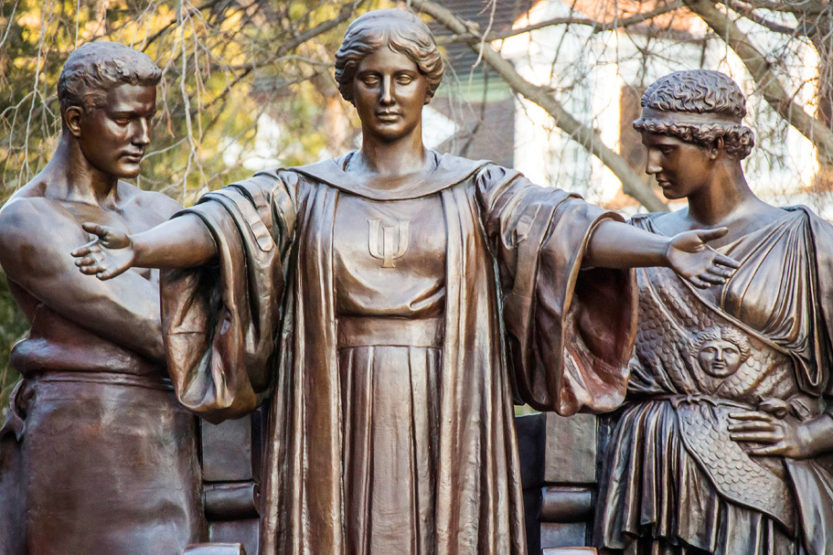
\includegraphics[width=0.44\textwidth]{alma.jpg}
    \caption{Alma Mater accompanied by Learning and Labor}
  \end{center}
\end{wrapfigure}
Founded in 1867, the University of Illinois at Urbana-Champaign (UIUC) has cultivated a long history of significant scientific discoveries and contributions. The theory of superconductivity, the invention of the transistor, the discovery of archaea, the fourth domain of life, and the first web browser are just some of the many breakthroughs that came out of UIUC. The famous Morrow Plots, established in 1876, became the first research crop field at a university and is still used today. Attendees might also be familiar with Blue Waters, one of the world’s fastest supercomputers. 
The UIUC Grainger College of Engineering has had sixteen Nobel Laureates in physics, including John Bardeen, the only scientist to ever win the award in physics twice. It also offers 15 different majors to almost 6000 undergraduate and 2500 graduate students. Of its twelve ranked majors, nine are ranked among the top 10 in the nation, and six of which remain ranked among the top 5 in their degree. Overall, the Grainger College of Engineering in Urbana-Champaign ranks sixth among the nation’s best undergraduate engineering programs. With more than 250 degrees for undergraduates and graduates and a multitude of first-class research facilities and resource, UIUC gives its nearly 45,000 students the ability to succeed. 

\subsection{UIUC ANS Student Chapter (ANS-UIUC)}
The ANS-UIUC maintains and develops a cohesive community of students in nuclear 
engineering. It also engages in education and outreach programs to teach 
members of the surrounding community about nuclear science. One of our most 
popular outreach programs is Engineering Open House (EOH), during which 
ANS-UIUC repeatedly earns awards for best presentation of a society. EOH is an 
annual event where members of the local community, from young children to 
senior adults, visit the engineering campus to learn more about STEM research. 
Membership is currently around 70-80 students and has been steadily growing. 
The chapter works to host events catering to nuclear, plasma, and radiological 
concentrations. Professional development plays a crucial role in student 
development, and it is the biggest part of member involvement at UIUC. 
Professional development activities range from tours of various facilities to 
pizza with campus visitors. Some of the past tours have included Clinton Power 
Station, Curium Pharma through UIUC Women In Nuclear, Oak Ridge National 
Laboratory, Analysis System (ANSYS) Inc, and Argonne National Laboratory. 
ANS-UIUC has historically been one of the best represented institutions at the 
annual student conference and hosting it is a tradition this chapter is eager 
to uphold. 


\begin{figure}[H]
  \centering
  \includegraphics[scale=0.15]{eoh1.JPG}
  \caption{Mouse Trap Chain Reaction at EOH 2019}
\end{figure}

\begin{figure}[H]
  \centering
  \begin{subfigure}{0.5\textwidth}
    \centering
    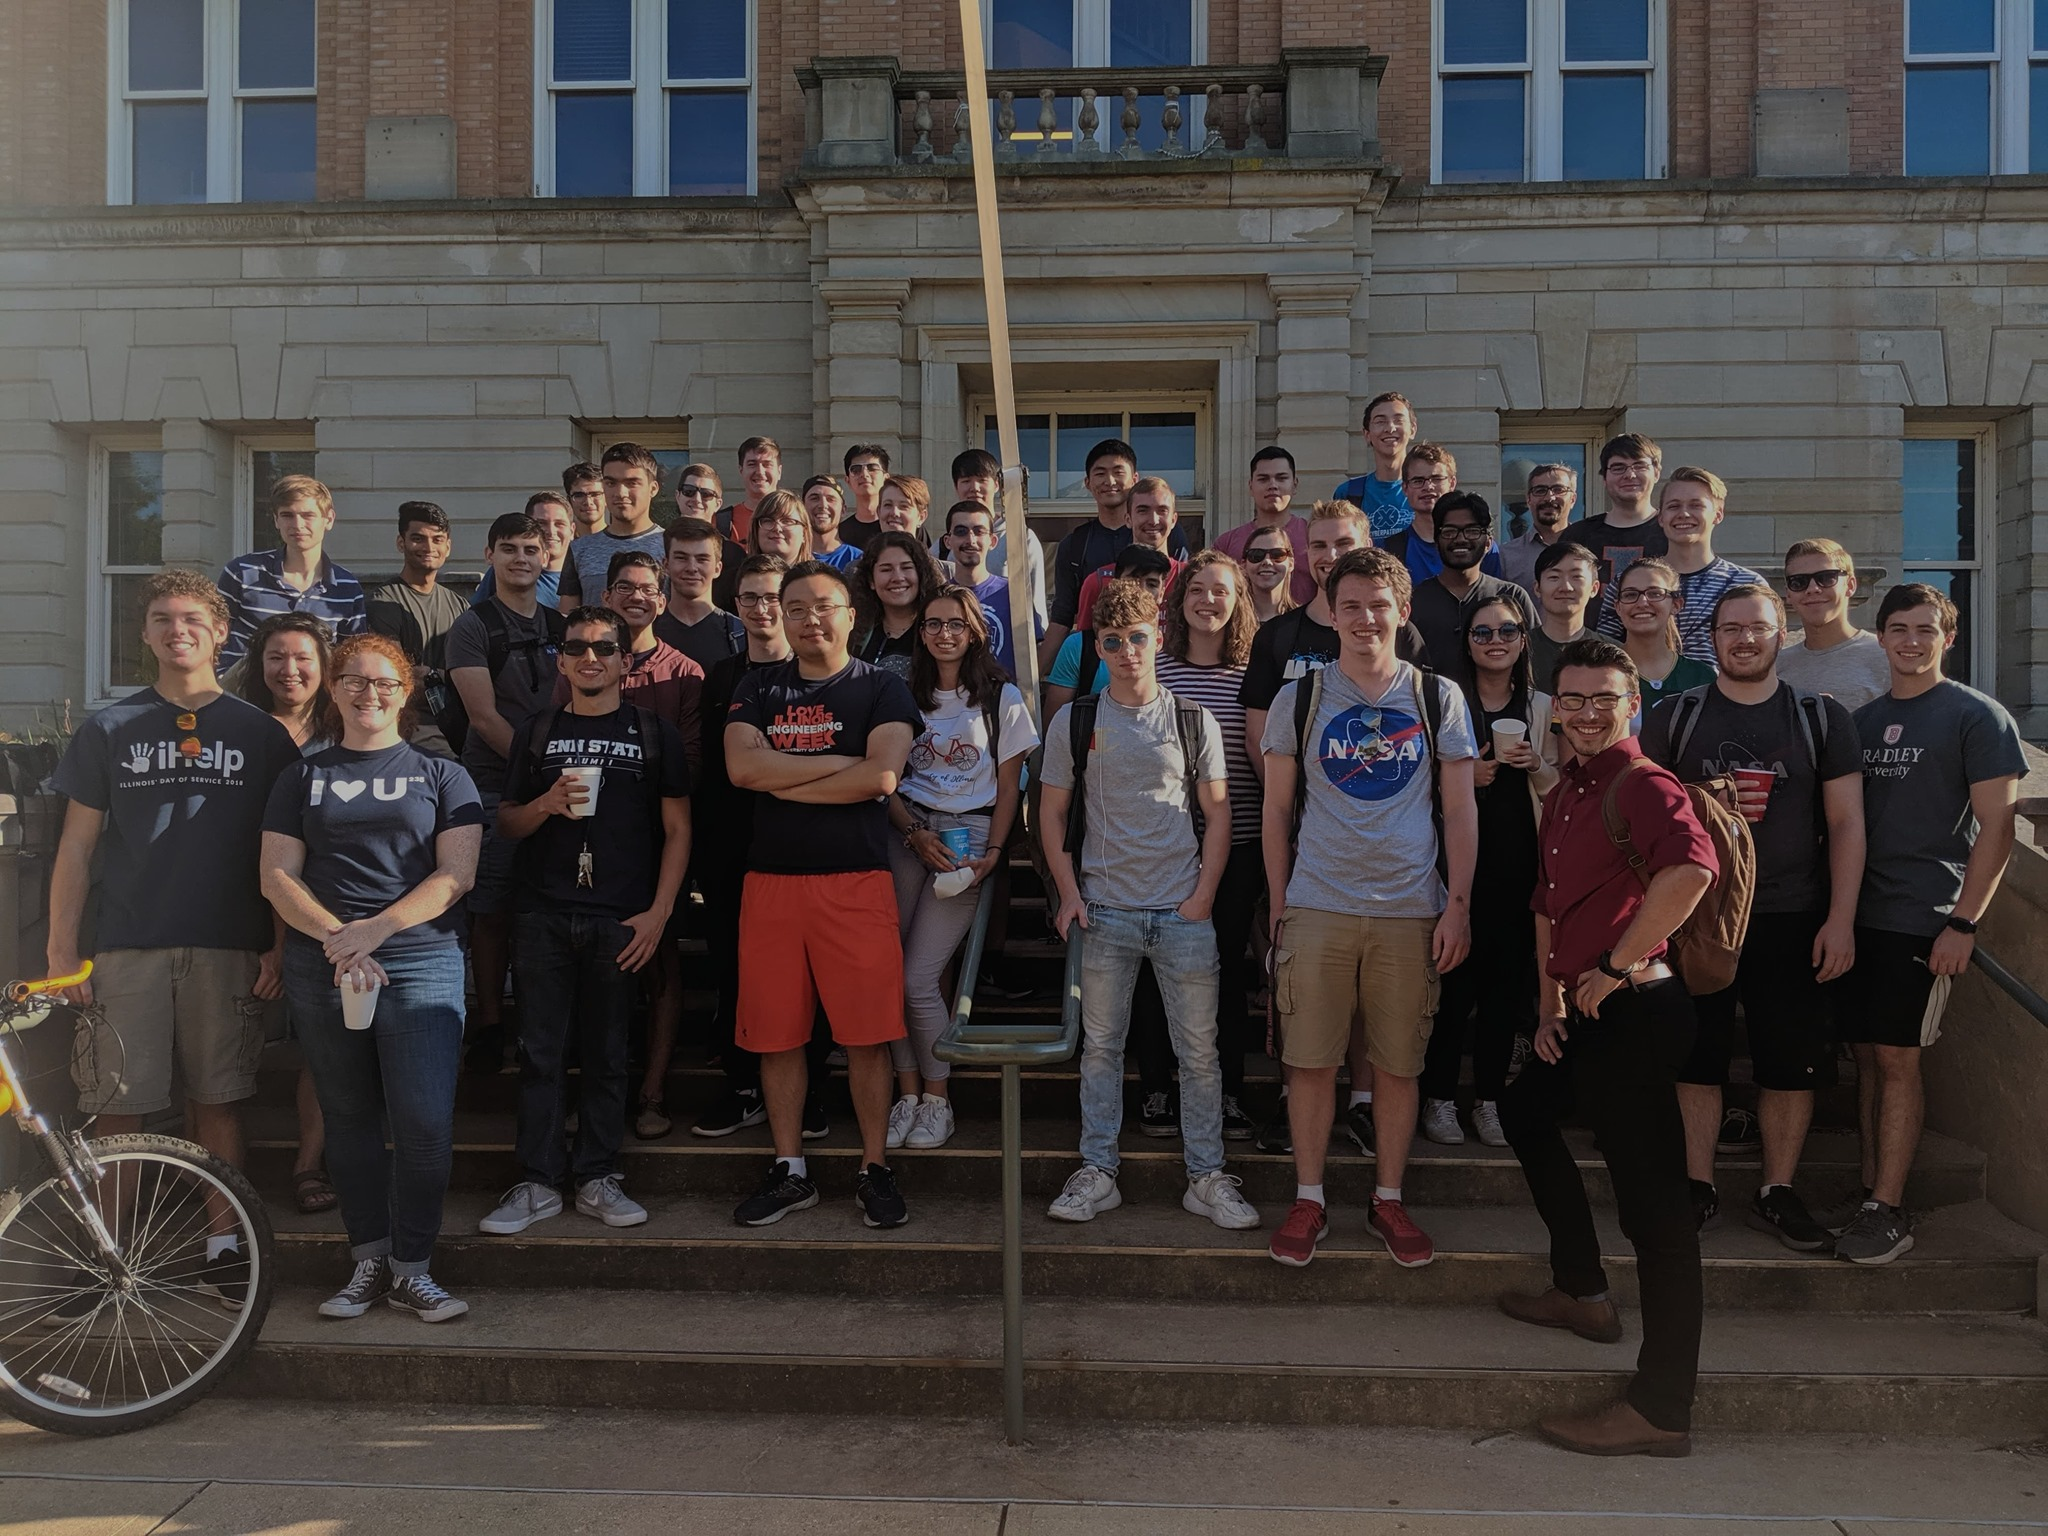
\includegraphics[width=8cm]{ans_uiuc_group.jpg}
    \subcaption{ANS Barbeque 2019}
  \end{subfigure}%
  \begin{subfigure}{0.5\textwidth}
    \centering
    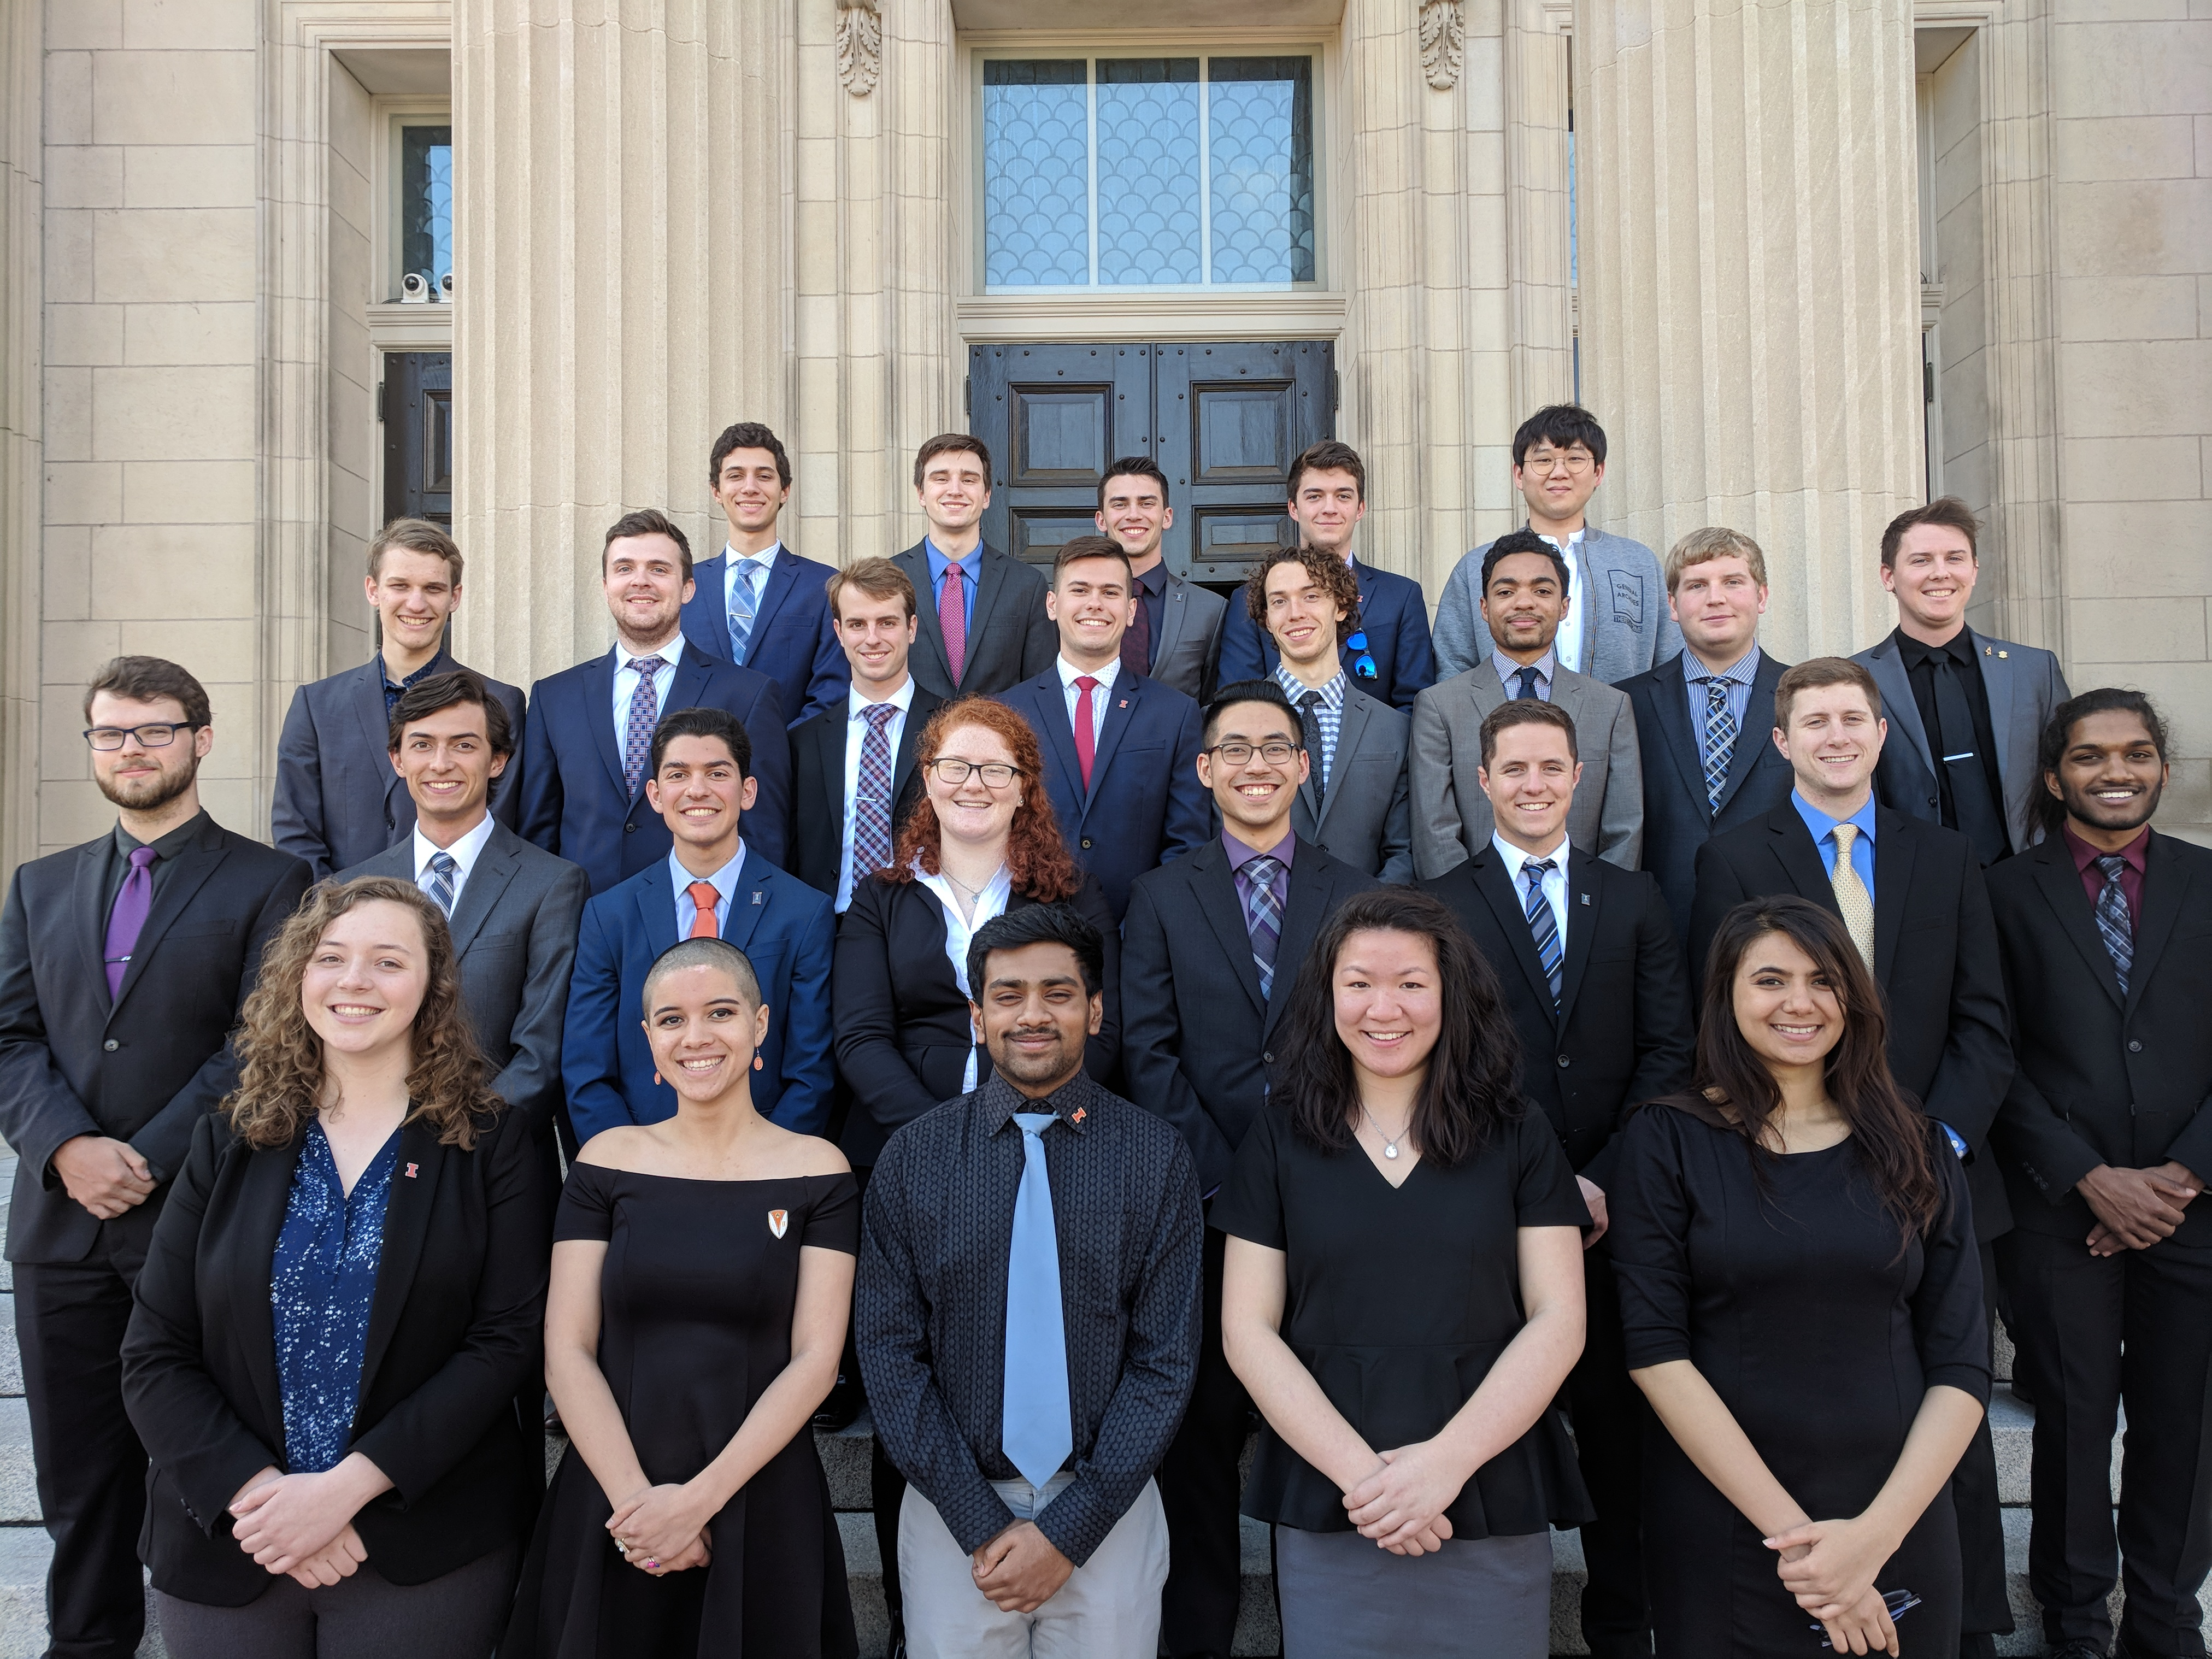
\includegraphics[width=8cm]{ans_conf_19.jpg}
    \subcaption{ANS Student Conference 2019 at VCU}
  \end{subfigure}   
  \caption{ANS Activities}
\end{figure} 

% \clearpage

\subsection{Research at UIUC}
Faculty and students in the Department of Nuclear, Plasma, and Radiological Engineering (NPRE) at Illinois conduct research in many areas of interest to the nuclear science community. Both graduate and undergraduate  students actively participate and make their own atomic contributions that will someday save the world.
Research programs in Nuclear, Plasma, and Radiological Engineering at the University of Illinois at Urbana-Champaign can be
broadly classified into five areas:
\begin{itemize}
        \item \textbf{Nuclear Power} (reactor physics, thermal hydraulics, fuel cycle, radiation transport, I\&C)
        \item \textbf{Plasma and Fusion} (modeling, plasma-material interactions)
        \item \textbf{Radiological Sciences} (detectors, imaging, health physics, medical applications)
        \item \textbf{Material Science} (nuclear fuels, structural materials)
        \item \textbf{Risk and Policy} (PRA, safety, energy, arms controls, disarmament, security)
\end{itemize}

These research areas are supported by a stellar faculty and world-class facilities, which 
will be briefly described below.

\subsubsection{Nuclear Power}
NPRE is well known for its pioneering research in the area of reactor power engineering. Graduates have gone on to leadership positions in industry, national laboratories, and academia. Research in the Nuclear Power concentration covers all aspects of power generation using nuclear energy on land, underwater (submarine), and in space. It is inherently interdisciplinary and relies on several branches of physics and engineering for design and analysis of large complex systems. These include aspects of reactor physics, reactor thermal-hydraulics, reactor safety, reliability and risk, instrumentation and control, training and education, human factors engineering, reactor materials, nonproliferation, and more. Safety standards and maintenance for existing reactors and new reactor designs are also explored by faculty in the department. Crosscutting areas of research include multi-physics and multi-scale modeling and simulation, high performance computing, reliability and risk, validation and verification, and uncertainty analysis. Recently, the University of Illinois declared a plan to be completely carbon-neutral by 2050. Nuclear power is the perfect candidate to help UIUC attain its carbon reduction and energy goals. Together, the University and the NPRE department are saving the world one atom at at time.

\subsubsection{Plasma Physics and Fusion Science}
\begin{wrapfigure}{r}{0.5\textwidth}
  \begin{center}
  \vspace{-\baselineskip}
    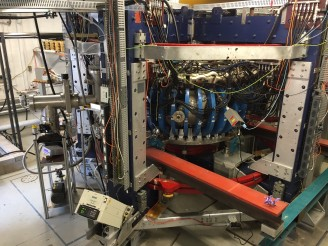
\includegraphics[width=0.48\textwidth]{hidra.png}
    \caption{The Hybrid Illinois Device for Research and Application (HIDRA)}
  \end{center}
\end{wrapfigure}
The Fusion and Plasma Physics research concentration in the NPRE department has a long history of work in the area of magnetic and inertial nuclear fusion as well as plasma engineering. NPRE is now one of the leading departments in plasma-material interactions with its Center for Plasma-Materials Interactions established by Prof. David Ruzic. Furthermore, in the past few years, two new faculty members have been added to this area: Prof. Davide Curelli and Prof. Daniel Andruzcyk. There are five research themes that spans the work in fusion and plasma physics: fusion materials, plasma-material interface (PMI) diagnostics, plasma-edge and PMI modeling, plasma nanosynthesis, and plasma sources and processing. The Hybrid Illinois Device for Research and Application (HIDRA) marks the newest addition to the team at CPMI. This device finished construction and achieved first plasma during the spring of 2016. \\


\subsubsection{Radiological Science}
Radiological engineering at UIUC strives to discover novel applications for ionizing radiation in biomedical research, homeland security, and nuclear safeguards. We have developed various gamma-ray, x-ray and neutron detectors, imaging devices, and novel algorithms for analyzing the data from these systems. These algorithms range from the use of so-called "big data" techniques applied to large sensor networks to advanced radiological imaging methods and image processing techniques for biomedical research. We work with physicists, biologists, chemists, material scientists, statisticians, and physicians around the world, to develop advanced diagnostic imaging and radiation-induced therapeutic approaches to address some of the most critical health care-related issues, such as cancer, cardiac diseases, diabetes and neurodegenerative disorders. We also work with organizations like the Departments of Defense, Energy, and Homeland Security and the International Atomic Energy Agency to deploy our research around the world to detect and identify the illicit movement of nuclear and radiological materials.

\subsubsection{Reliability and Risk Analysis}
Risk analysis represents the pinnacle of interdisciplinary research and education. Following the Three Mile Island disaster in 1979, Probabilistic Risk Assessment (PRA) has become a key pillar of the risk-informed nuclear regulatory framework, and is now a requirement for every nuclear power plant in the United States. Enhancing the prevention of catastrophic technological accidents and the protection of the environment requires advancement in multidisciplinary PRA. It demands the development of a common vocabulary within diverse engineering and social science domains in order to address risks that emerge from the interface of social and technical systems.


\subsubsection{Materials Science}
Materials science research includes investigations of the mechanical properties of cladding and other structural components, and heat exchanger materials. Advanced microanalysis techniques are often employed to perform nano-scale interrogation of deformation, precipitation, and chemical segregation studies, etc. Ion beam bombardment of materials is often used with these techniques to simulate fast neutron displacement cascade damage. Fuel performance modeling, molecular dynamics, and kinetic Monte Carlo simulations complement these experimental activities. The department also has strong efforts related to the study of nuclear fuel such as urania, including mass transport and mechanical property studies. The department also studies hydrogen in metals, including hydride phase formation and solute dislocation pipe diffusion.


\subsubsection{Reliability and Risk Analysis}
\begin{wrapfigure}{r}{0.5\textwidth}
  \begin{center}
  \vspace{-\baselineskip}
    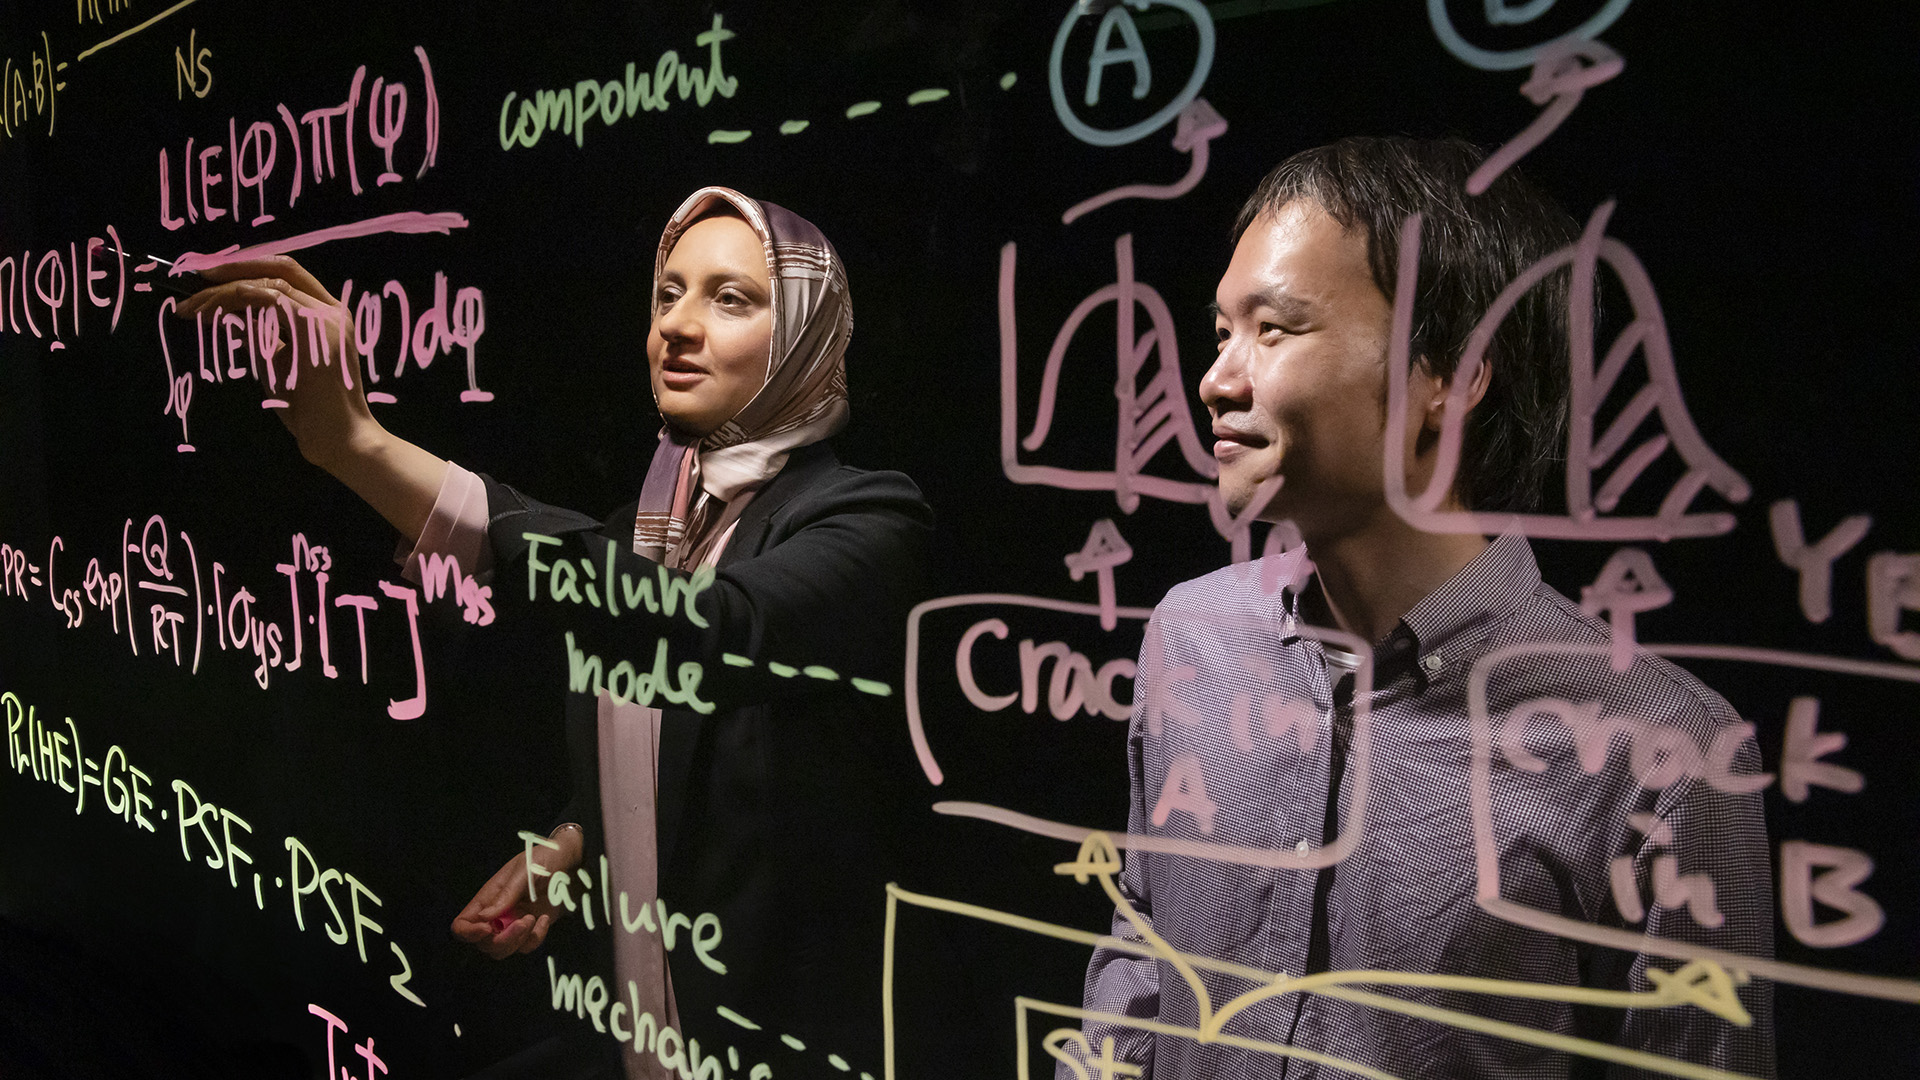
\includegraphics[width=0.48\textwidth]{mohaghegh.jpg}
    \caption{Prof. Zahra Mohaghegh is an Assistant Professor in Nuclear, 
          Plasma, and Radiological Engineering and director of the 
          Socio-Technical Risk Analysis (SoTeRiA) Research Laboratory.}
  \end{center}
\end{wrapfigure}
Risk analysis represents the pinnacle of interdisciplinary research and education. Following the Three Mile Island disaster in 1979, Probabilistic Risk Assessment (PRA) has become a key pillar of the risk-informed nuclear regulatory framework, and is now a requirement for every nuclear power plant in the United States. Enhancing the prevention of catastrophic technological accidents and the protection of the environment requires advancement in multidisciplinary PRA. It demands the development of a common vocabulary within diverse engineering and social science domains in order to address risks emerging from the interface of social and technical systems.
\subsubsection{NPRE Research Groups and Laboratories}
The faculty, pictured in Figure \ref{fig:faculty} support the above areas of 
expertise in the collaborations and facilites discussed below.

\begin{figure}[htbp]
        \begin{center}
                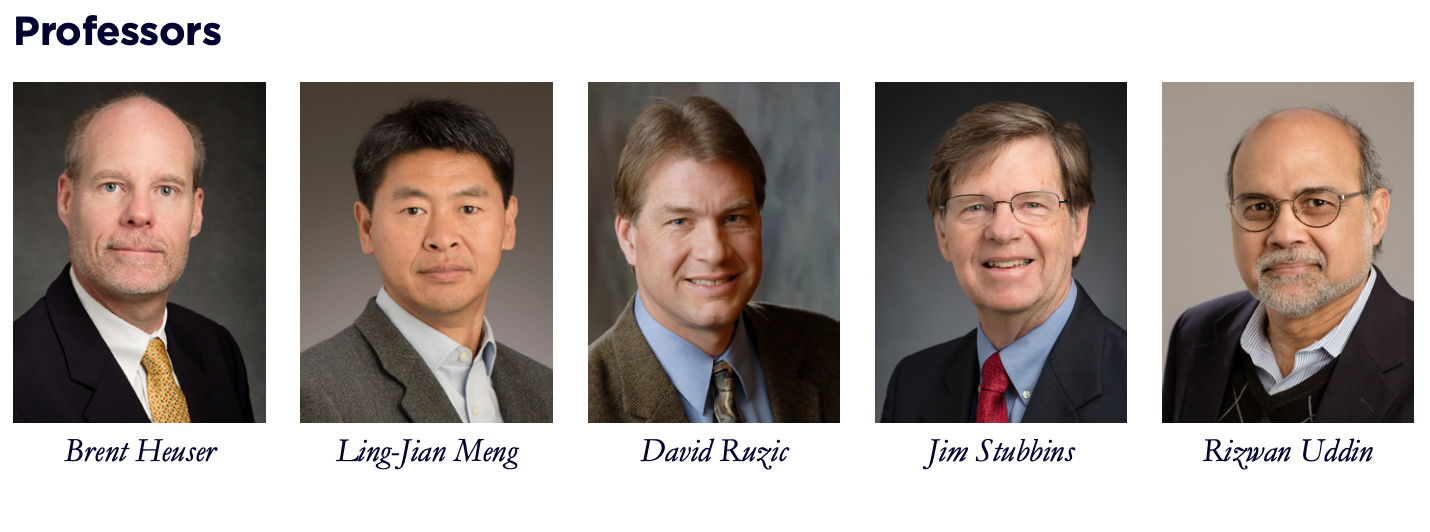
\includegraphics[width=0.75\textwidth]{./images/full.png}
                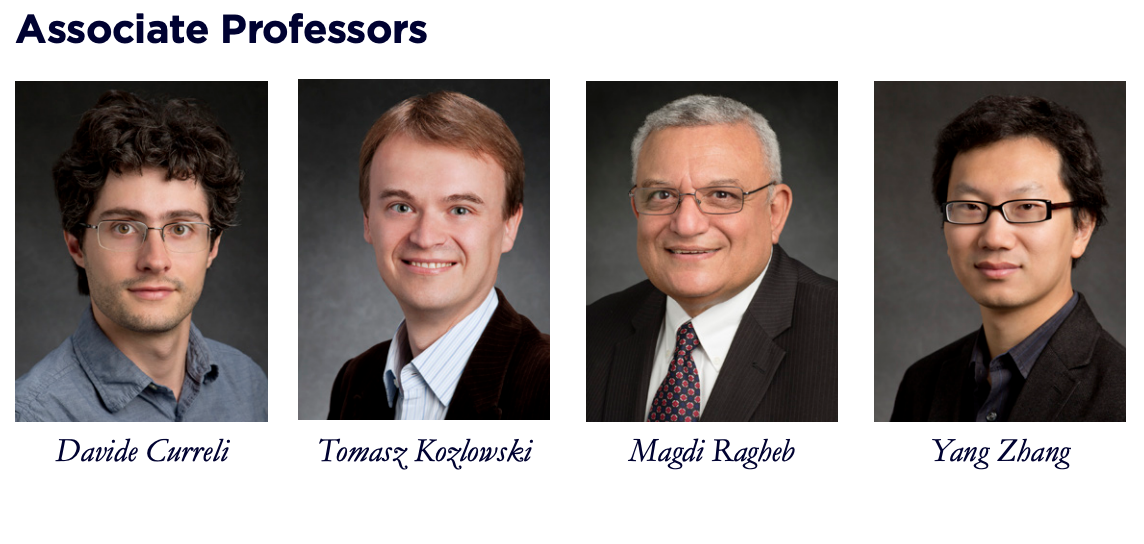
\includegraphics[width=0.6\textwidth]{./images/associate.png}
                
\includegraphics[width=0.6\textwidth]{./images/assistant.png}
                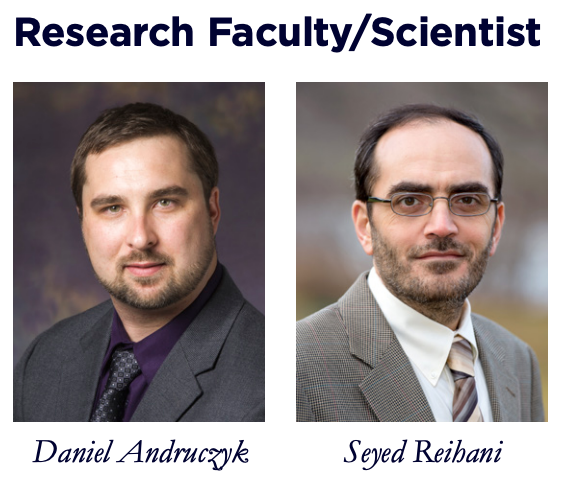
\includegraphics[width=0.3\textwidth]{./images/research.png}
        \end{center}
        \caption{Faculty in Nuclear, Plasma, and Radiological Engineering  at 
        the University of Illinois at Urbana-Champaign.}
        \label{fig:faculty}
\end{figure}

\begin{itemize}
  \item \textbf{Advanced Reactors and Fuel Cycles (ARFC)} - \textit{Dr. Kathryn Huff}\\
  The ARFC group seeks to advance the safety and sustainability of nuclear energy production through improved reactor designs, fuel cycle strategies, and waste management techniques. In the area of advanced reactors, their work focuses on extending current simulation tools with features essential to advanced reactor multiphysics. In the context of the broader nuclear fuel cycle, the ARFC group emphasizes modeling, simulation, and analysis of the global nuclear fuel cycle, with an emphasis on sustainability. A crosscutting theme of our research is an emphasis on advancing methods and software for computational nuclear engineering. Accordingly, the Advanced Reactors and Fuel Cycles group is proud to be affiliated with the University of Illinois National Center for Supercomputing Applications and its Blue Waters computing facility.
  \item \textbf{Virtual Education and Research Laboratory (VERL)} - \textit{Dr. Rizwan Uddin}\\
  The VERL group focuses on the development of innovative numerical methods and their implementation on high performance computing machines. Research efforts center on problems in nuclear engineering, with emphasis on thermal-hydraulics and reactor physics.

  \item \textbf{Analysis of Reactor Transients and Stability (ARTS)} - \textit{Dr. Tomasz Kozlowski}\\
  The ARTS group performs deterministic safety analysis by developing and validating advanced methods to accurately determine reactor safety margins and reactor behavior. By performing high-fidelity numerical predictions of the reactor behavior in abnormal transient scenarios of safety significance, their work supports the nuclear reactor safety analysis, and increases the fidelity of primary system simulation. This approach is at the heart of nuclear power’s excellent safety record – always striving to improve current tools and methods.

  \item \textbf{Center for Plasma-Material Interactions (CPMI)} - \textit{Dr. David Ruzic}\\
  The primary objective of CPMI is the study of plasma-material interactions relevant to fusion, semiconductor manufacturing, and plasma processing through a combination of experimental and computational means. CPMI has facilities for the study of fusion materials, High Power Impulse Magnetron Sputtering (HiPIMS), liquid metals, Extreme Ultraviolet Lithography (EUVL),  laser-material interactions, and more. Projects are supported by both government and commercial partners to further the application and knowledge of plasma physics. The facility recently finished the construction of the HIDRA fusion device, which is a stellarator-tokamak machine hybrid machine used to study plasma-materials interactions.  HIDRA is currently run by Dr. Daniel Andruczyk.

  \item \textbf{Materials Science} - \textit{Dr. James F. Stubbins}\\
  The group investigates a wide variety of topics within the realm of materials research including mechanical properties, microstructural evaluations, plus radiation damage investigations, and modeling. Materials such as copper alloys nickel-based alloys, stainless steels, ferritic steels, and silicon-carbide composites are studied using a variety of analytical techniques electron microscopy and spectroscopy.


  \item \textbf{Non-Equilibrium Matter Laboratory} - \textit{Dr. Yang Zhang}\\
  This laboratory focuses on the study of non-equilibrium matter, with particular emphasis on liquids and soft matter, using integrated neutron and synchrotron light experimental probes and atomistic modeling and simulation. The structure and dynamics of these systems are either inherently complex or driven away from equilibrium by extreme conditions. In particular, their current interests include a range of fundamental and technical problems involving slow phenomena and rare events, such as: materials far from equilibrium and in extreme environments; extreme properties of liquids; and glassy or jammed soft matters.

  \item \textbf{Radiation Imaging Group} - \textit{Dr. Ling Jian Meng}\\
  Research is on developing radiation sensor and systems for visualizing the distribution of radioactivity in surrounding objects, patients, and small lab animals etc. Current emphasis includes (a) developing novel radiation sensors for detecting X-ray, gamma rays and neutrons, and (b) developing nuclear techniques for detecting and imaging a tiny amount radiolabeled molecules inside small lab animals.

  \item \textbf{Socio-Technical Risk Analysis (SoTeRiA)} - \textit{Dr. Zahra Mohaghegh}\\
  The Socio-Technical Risk Analysis (SoTeRiA) Laboratory is evolving Probabilistic Risk Assessment (PRA) by explicitly incorporating the underlying science of accident causation into risk scenarios. SoTeRiA laboratory has pioneered two key areas of theoretical and methodological innovations: (1) spatio-temporal causal modeling of social and physical failure mechanisms in PRA, and (2) the fusion of big data analytics with PRA. The Lab’s current projects include: Fire PRA; Location-specific Loss- Of-Coolant Accident (LOCA) Frequency Estimations; Risk-Informed Resolution of Generic Safety Issue 191; Human and Organizational Influences on System Risk; Risk-Informed Regulation; and Risk-Informed Emergency Preparedness, Planning and Response.

  \item \textbf{Laboratory: High Temperature Environmental Exposure Lab} - \textit{Dr. Brent Heuser}\\
  A simultaneous thermal analyzer with combined thermogravimetric and differential scanning calorimetry function is housed in this laboratory. The response of LWR fuel cladding materials in high temperature steam environments for improved accident tolerance is currently of interest.

  \item \textbf{Laboratory: Nuclear Materials Fabrication and Studies Lab} - \textit{Dr. Brent Heuser}\\
  The Radiation Detection and Imaging Lab focuses on developing non-invasive imaging technology for use in preclinical medical research. Many of their current endeavors focus on developing semiconductor Single Photon Emission Computed Tomography (SPECT) and Positron Emission Tomography (PET). These works challenge the current state of the art for spatial resolution and system sensitivity. The use of highly pixelated CdTe detectors has driven their work to break into a spatial resolution on the order of 300 microns for both PET and SPECT. Their work in SPECT has also challenged the limits of aperture sensitivity through the engineering of the compound-eye aperture.

  \item \textbf{Laboratory: Multiphase Thermo-fluid Dynamics Lab} - \textit{Dr. Caleb Brooks}\\
  This group performs experiments related to thermal hydraulics and multiphase flow. Phenomena studied include boiling, condensation, critical heat flux, natural circulation, two-phase flow instabilities, bubble dynamics, and two-phase transport. Utilizing advanced instrumentation, data from these experiments are used in model development and validation of computational tools.
  \item \textbf{Laboratory: Nuclear Measurements Laboratory} - \textit{Dr.  Angela DiFulvio}\\ The lab is equipped with a Cf-252 source and a D-T neutron generator with an emission rate of ~1E7 and ~1E8 neutrons/s, respectively. The neutron flux density is well-characterized in energy and intensity employing various instruments, including multisphere spectrometers, ionization chambers, long counters, and scintillators, calibrated to primary reference standards, which enable the detection of neutrons via scattering of protons or via fission of uranium nuclei.
\end{itemize}
